\usepackage{graphicx}
\newpage
\thispagestyle{fancy}
\vspace{\fill}

\subsection{Pressão manual no Porta Manta}
\begin{figure}
    \centering
    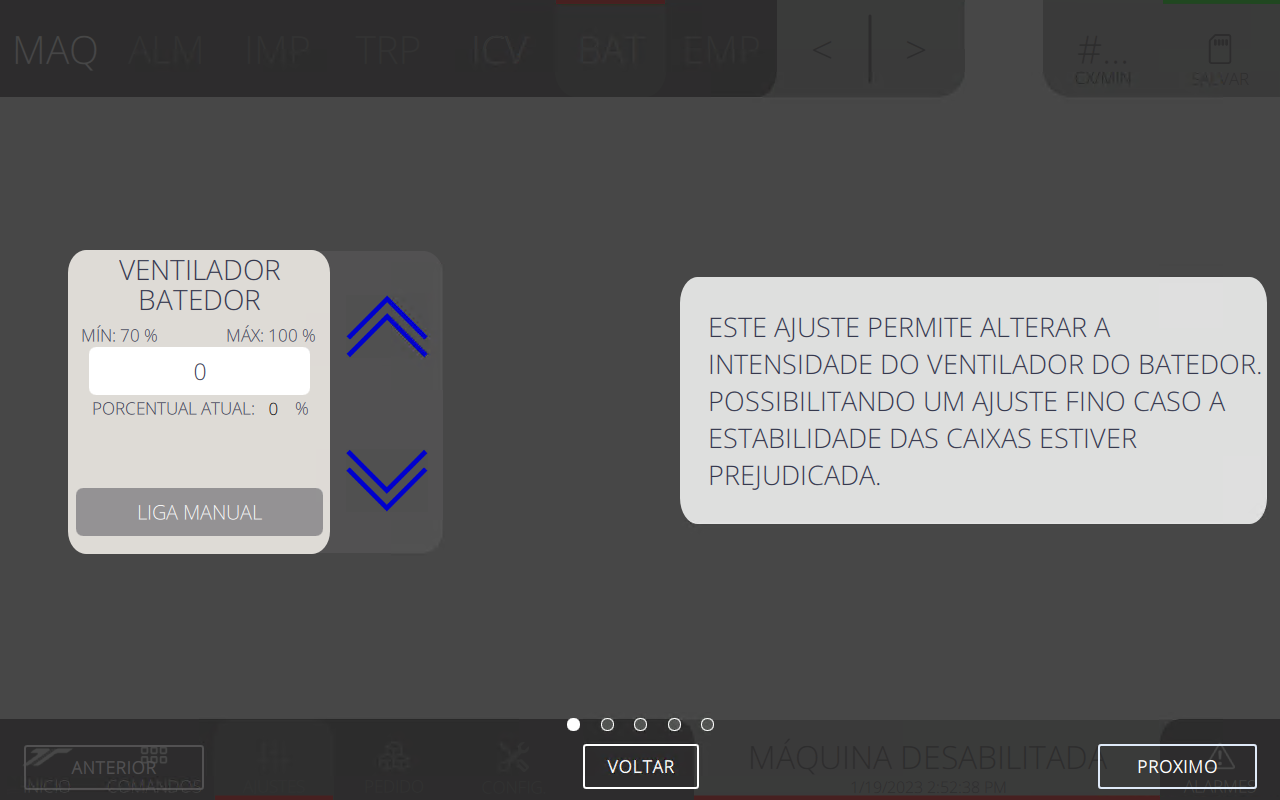
\includegraphics[width=480,height=300]{imagesICV/06-dryCutter/settings/e-1}
    \caption{Pressão manual no Porta Manta}
\end{figure}
\newpage
\thispagestyle{fancy}
\vspace{\fill}

\subsection{Pressão manual no Porta Manta}
\begin{figure}
    \centering
    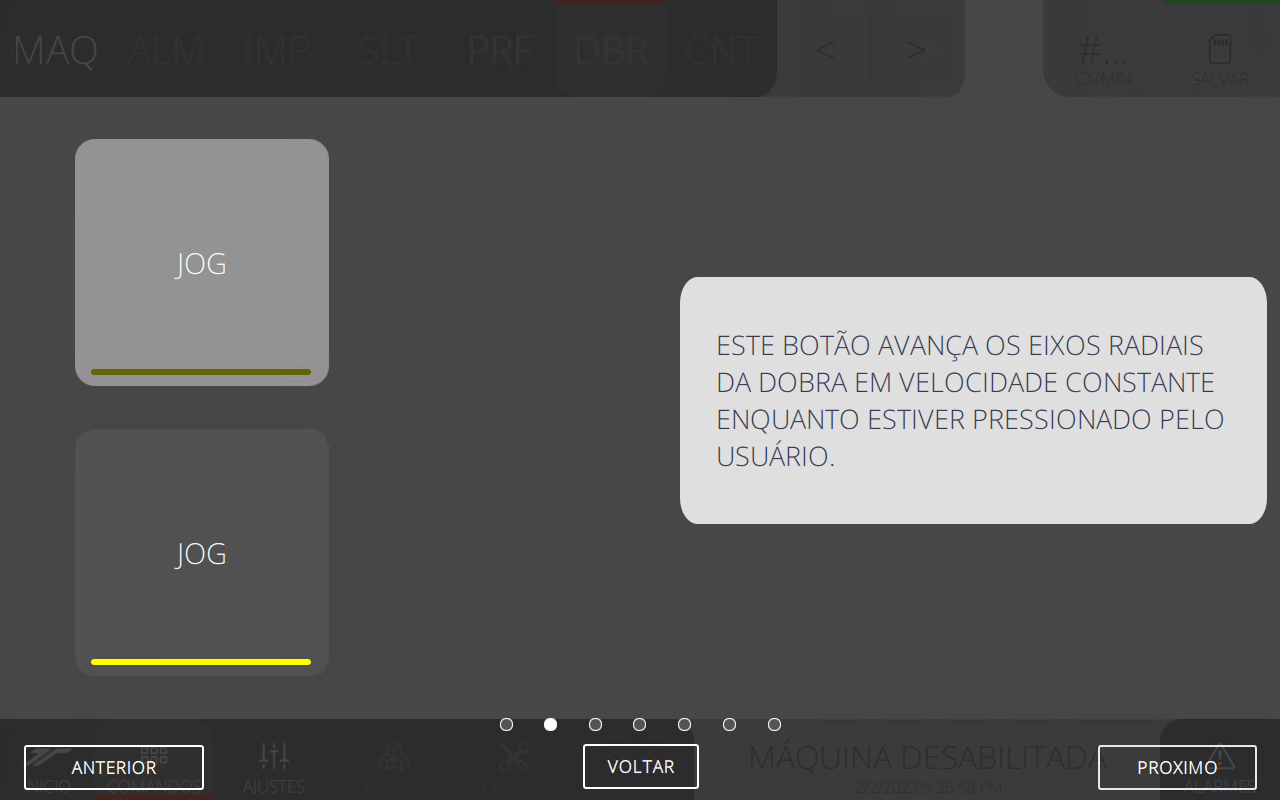
\includegraphics[width=576,height=360]{imagesICV/06-dryCutter/settings/e-2}
    \caption{Pressão manual no Porta Manta}
\end{figure}
\newpage
\thispagestyle{fancy}
\vspace{\fill}

\subsection{Radial Porta Ferramenta}
\begin{figure}
    \centering
    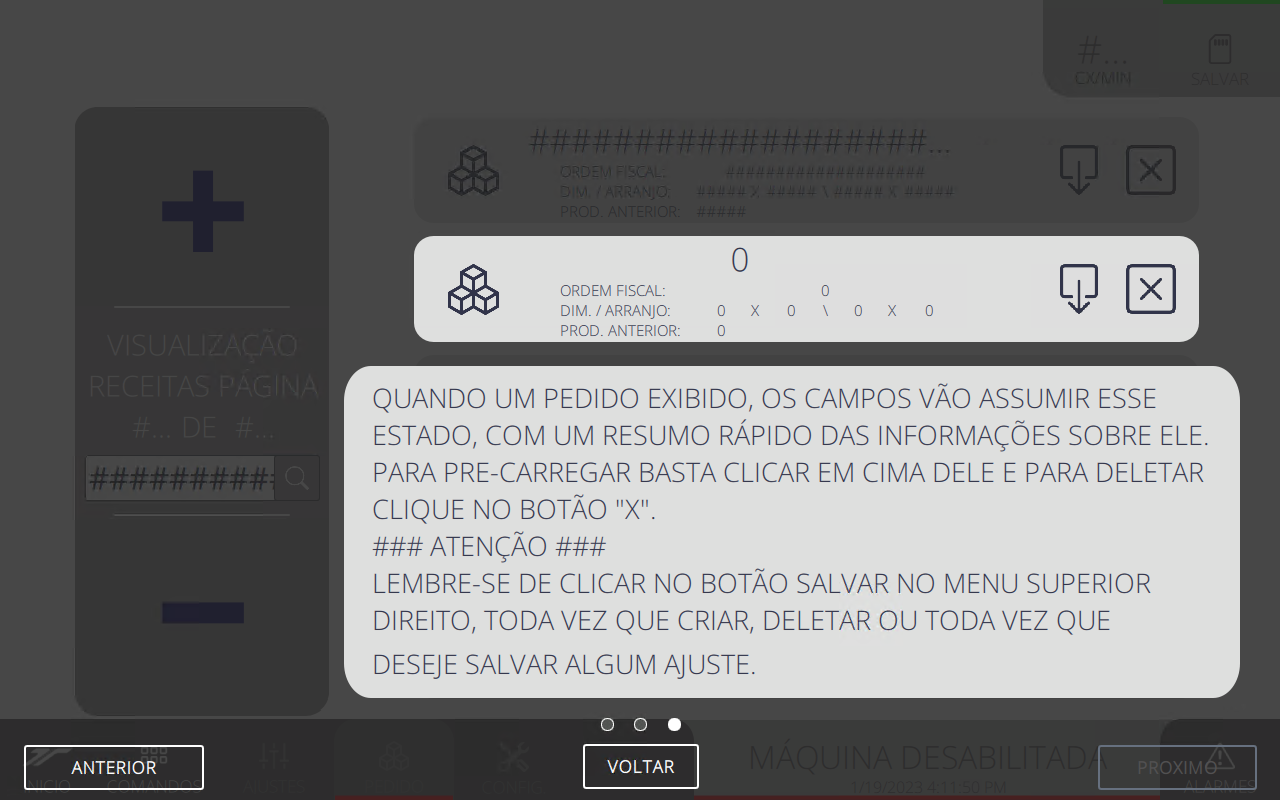
\includegraphics[width=576,height=360]{imagesICV/06-dryCutter/settings/e-3}
    \caption{Radial Porta Ferramenta}
\end{figure}
\newpage
\thispagestyle{fancy}
\vspace{\fill}

\subsection{Perímetro da Manta}
\begin{figure}
    \centering
    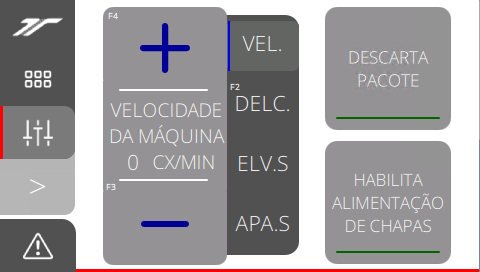
\includegraphics[width=576,height=360]{imagesICV/06-dryCutter/settings/e-4}
    \caption{Perímetro da Manta}
\end{figure}]
\newpage
\thispagestyle{fancy}
\vspace{\fill}

\subsection{Setpoint pressão Porta Manta afastado}
\begin{figure}
    \centering
    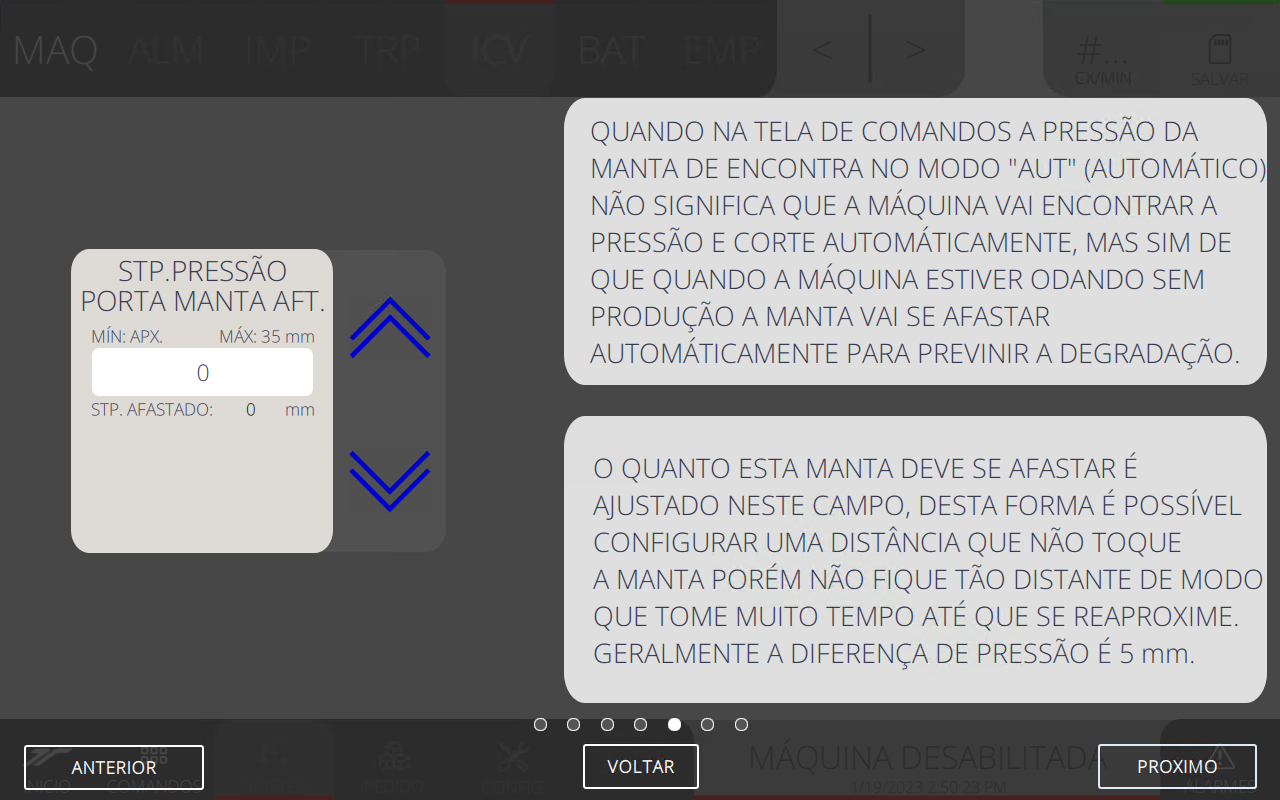
\includegraphics[width=576,height=360]{imagesICV/06-dryCutter/settings/e-5 COM ERRO DE DIGITAÇÃO}
    \caption{Setpoint pressão Porta Manta afastado}
\end{figure}
\newpage
\thispagestyle{fancy}
\vspace{\fill}

\subsection{Setpoint pressão Porta Manta aproximado}
\begin{figure}
    \centering
    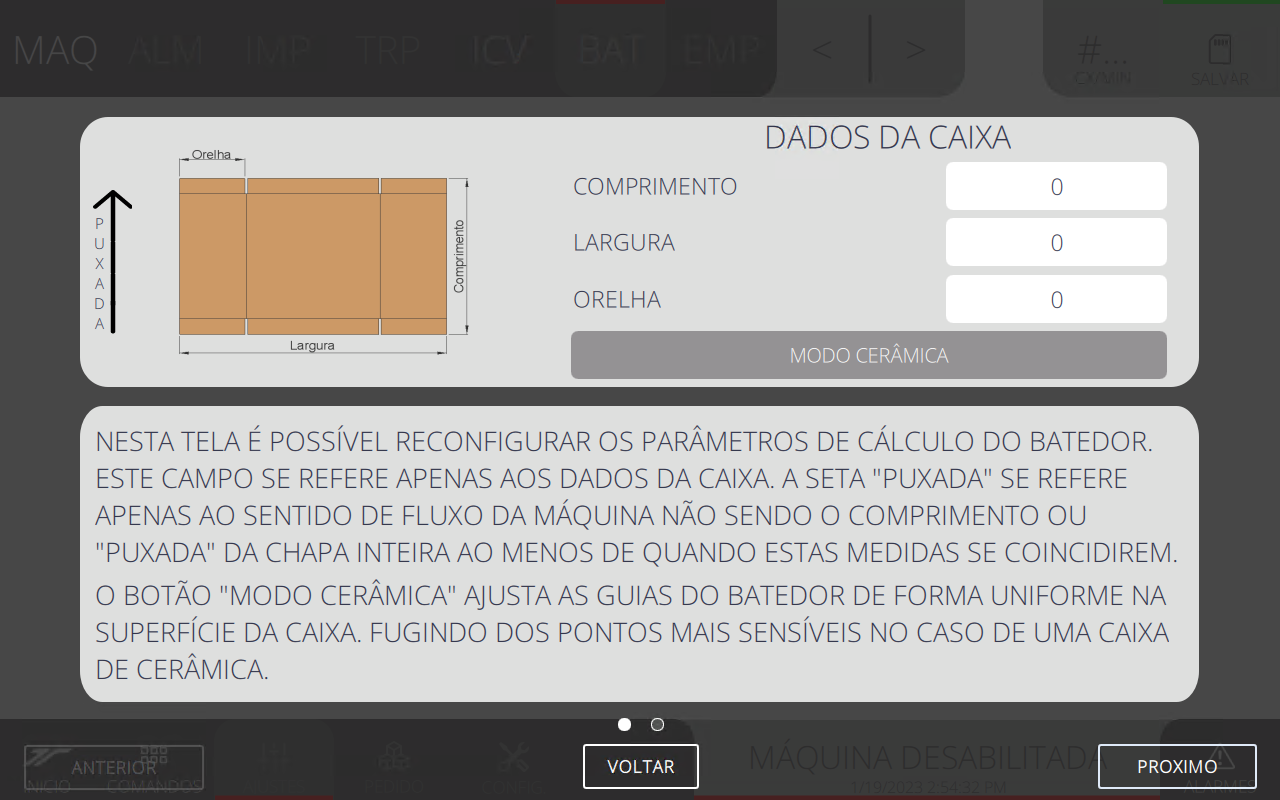
\includegraphics[width=576,height=360]{imagesICV/06-dryCutter/settings/e-6}
    \caption{Setpoint pressão Porta Manta aproximado}
\end{figure}
\newpage
\thispagestyle{fancy}
\vspace{\fill}

\subsection{Axial Porta Ferramenta}
\begin{figure}
    \centering
    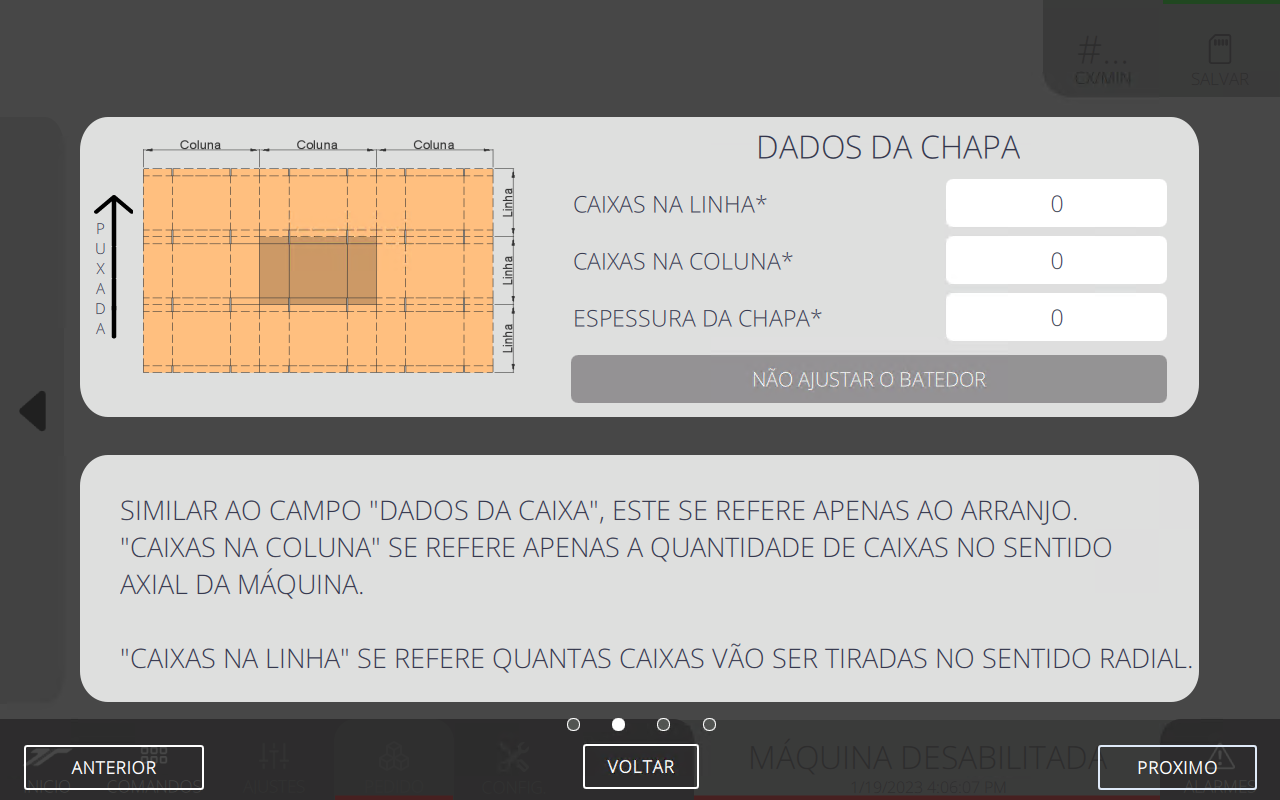
\includegraphics[width=576,height=360]{imagesICV/06-dryCutter/settings/e-7}
    \caption{Axial Porta Ferramenta}
\end{figure}
